\chapter{Remote water metering system overview}

The proposed system consists of software and hardware components shown in \ref{fig:rwm}.


\section{Opto-coupling with the existing meter}

We decided to glue an opto-electronical device right on top of the revolving disc segment.
An infrared is reflected from the disc as it passes underneath the sensor. One revolution equals \SI{10}{\litre}. The details on how
this signal is translated into a digitized pulse stream is discussed later in this document.

\section{Off-grid electricity production}

Since the existent water meter is installed inside a water gully with no electricity outlet in the vicinity,
the energy required to operate the system must be produced by the installation.
We explore two different approaches:
\begin{enumerate}
    \item a small solar panel capable of delivering \SI{10}{\watt} peak power.
    \item a microturbine connected to a nearby  reservoir overflow outlet capable of delivering approx. \SI{8}{\volt} @ \SI{8}{\milli\ampere}.
\end{enumerate}


\begin{figure}[h]
    \centering
    \begin{subfigure}[b]{0.45\textwidth}
        \centering
        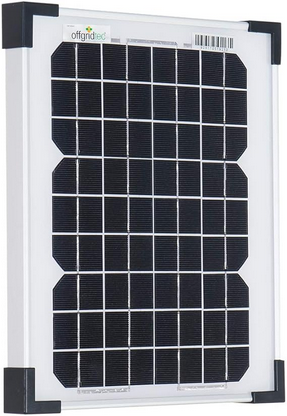
\includegraphics[width=.3\linewidth]{solarpanel}
        \subcaption{solar panel (10 W)}
        \label{fig:sp}
    \end{subfigure}
    \hfill
    \begin{subfigure}[b]{0.45\textwidth}
        \centering
        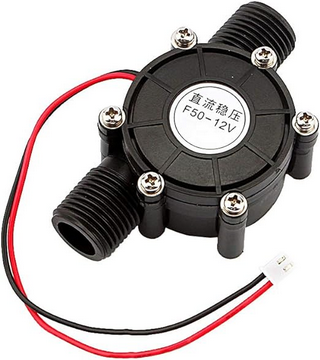
\includegraphics[width=.3\linewidth]{microturbine}
        \subcaption{consumer microturbine (60 mW)}
        \label{fig:mt}
    \end{subfigure}
    \caption{Inexpensive off-grid power production}
    \label{fig:ewm}
\end{figure}

Currently, we use two solar panels oriented south and west, respectively. The microturbine requires a different circuit in order to charge
a LiPo battery. We will discuss this circuit in a different article. Also, note that the depicted model is rather a toy and most likely
unsuited for an application in production. We also noted that the additional wiring and electrical trench provision are probably too high
a cost in our use case. But we do think, that it would be interesting to gather more data and experience with this kind of inexpensive
consumer products because in some situations - and for some village budgets - this might be the only choice.

The two solar panels are located in a rather shady forest area at a distance  of 15 m from the gully
housing the water meter and the sensor hardware.

\begin{figure}[h]
    \centering
    \includegraphics[width=0.5\textwidth]{site}
    \caption{Solar panel configuration}
    \label{fig:x}
\end{figure}


\section{MQTT}

\href[]{https://mqtt.org/}{MQTT} is a widely used protocol to connect embedded systems - things - to the internet.
It is ideally suited (but not limited to) for applications where relatively low data volumes must be transmitted in regular time intervals, like for
example temperature sensors.
In our case, we need to transmit readings from the water meter as often as the available amount of energy allows it.
Currently, this amounts to one transmission per day, but there is potential for more frequent transmissions, as we will
discuss later in this paper.
Recall, that we want to react rapidly to potential leaks.

MQTT is \href[]{https://mqtt.org/}{touted} as being \textquote{lightweight}:

\begin{displayquote}
    MQTT is an OASIS standard messaging protocol for the Internet of Things (IoT).
    It is designed as an extremely lightweight publish/subscribe messaging transport that is ideal for
    connecting remote devices with a small code footprint and minimal network bandwidth.
\end{displayquote}

Note that the cloud based broker we use is not free of charge. Currently, we occur between 5 and 10 USD in transmission costs per month. This
is not negligible and points to the necessity to replace the GSM network layer with a locally provided infrastructure, wherever possible. One way to do so
would be a LoRaWAN-type protocol based on the 867 Mhz band. Another option is to use a service like  \href[]{https://ngrok.com/}{ngrok} to securely expose a locally
hosted MQTT broker to the Internet.


\section{Data retrieval and storage}

After the meter readings have been uploaded to the MQTT broker, we need to retrieve it to a local workstation or server for storage, display
and further analysis.
We have developed a Java based application that runs as a Linux daemon on an always-on small form factor PC in the office of a local resource manager.
This software connects to the MQTT broker, downloads the latest readings and stores them to a local database.
User relevant data is also stored to a cloud-based database, from where the data can be displayed on a globally accessible internet website
dedicated to the resource management of a group of communities.
More comprehensive data is further published to a local MQTT broker. We use \href[]{https://www.home-assistant.io/}{Home Assistant} as
a highly configurable admin dashboard.
The daemon software also monitors consumption thresholds.
Unusually high average readings potentially implying a leak will trigger an SMS alert and an email alert.

The design and implementation of this software will be discussed in a different paper.



In this chapter we will highlight some elements shown Fig \ref{fig:rwm}, specifically those in the Embedded System part.

\begin{figure}[h]
    \centering
    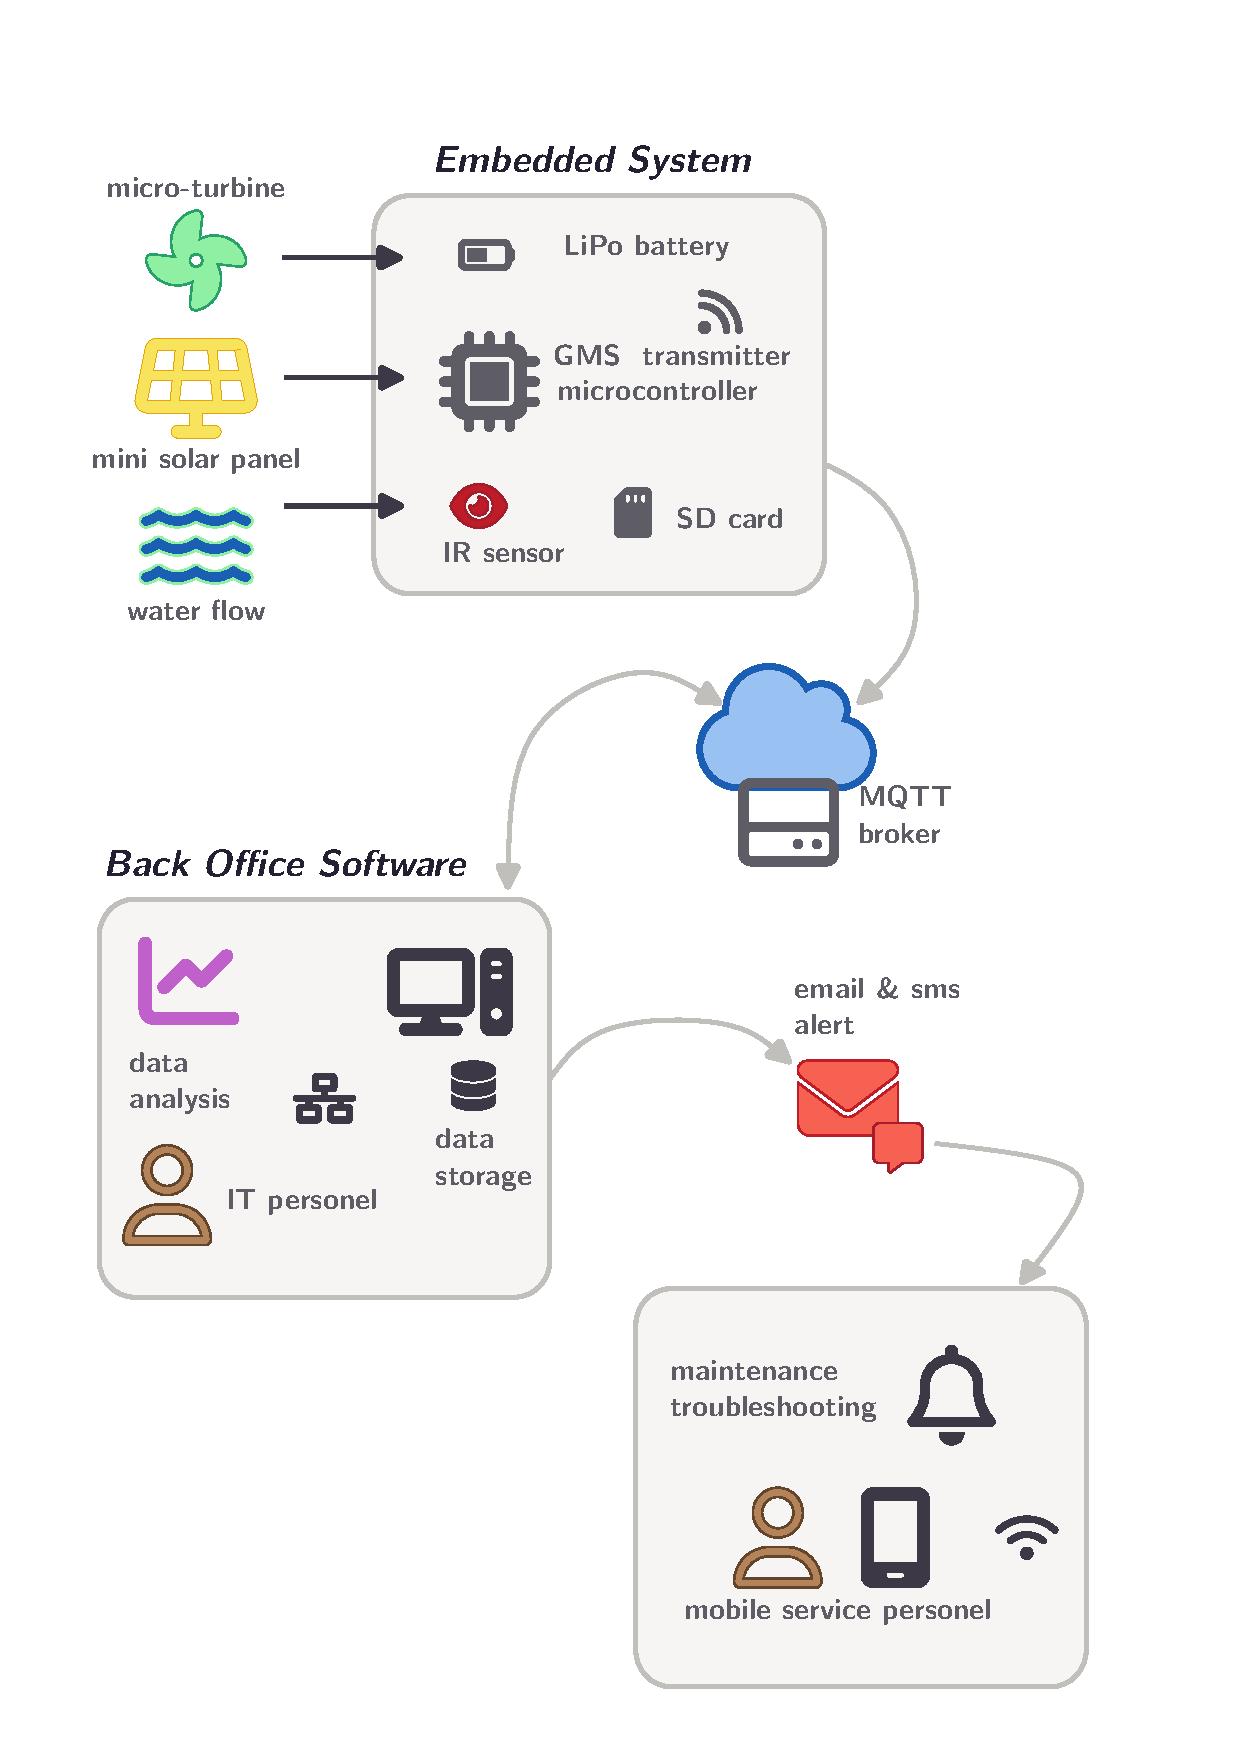
\includegraphics[scale=0.6]{overview}
    \caption{Remote Water Meter system overview}
    \label{fig:rwm}
\end{figure}